\subsection{Performance}



\begin{figure*}[t]

  \begin{subfigure}[b]{\textwidth}
          \centering
          
\includegraphics[width=0.4\textwidth]{data/legend.pdf}
  \end{subfigure}

  \begin{subfigure}[b]{0.5\textwidth}
      \centering
      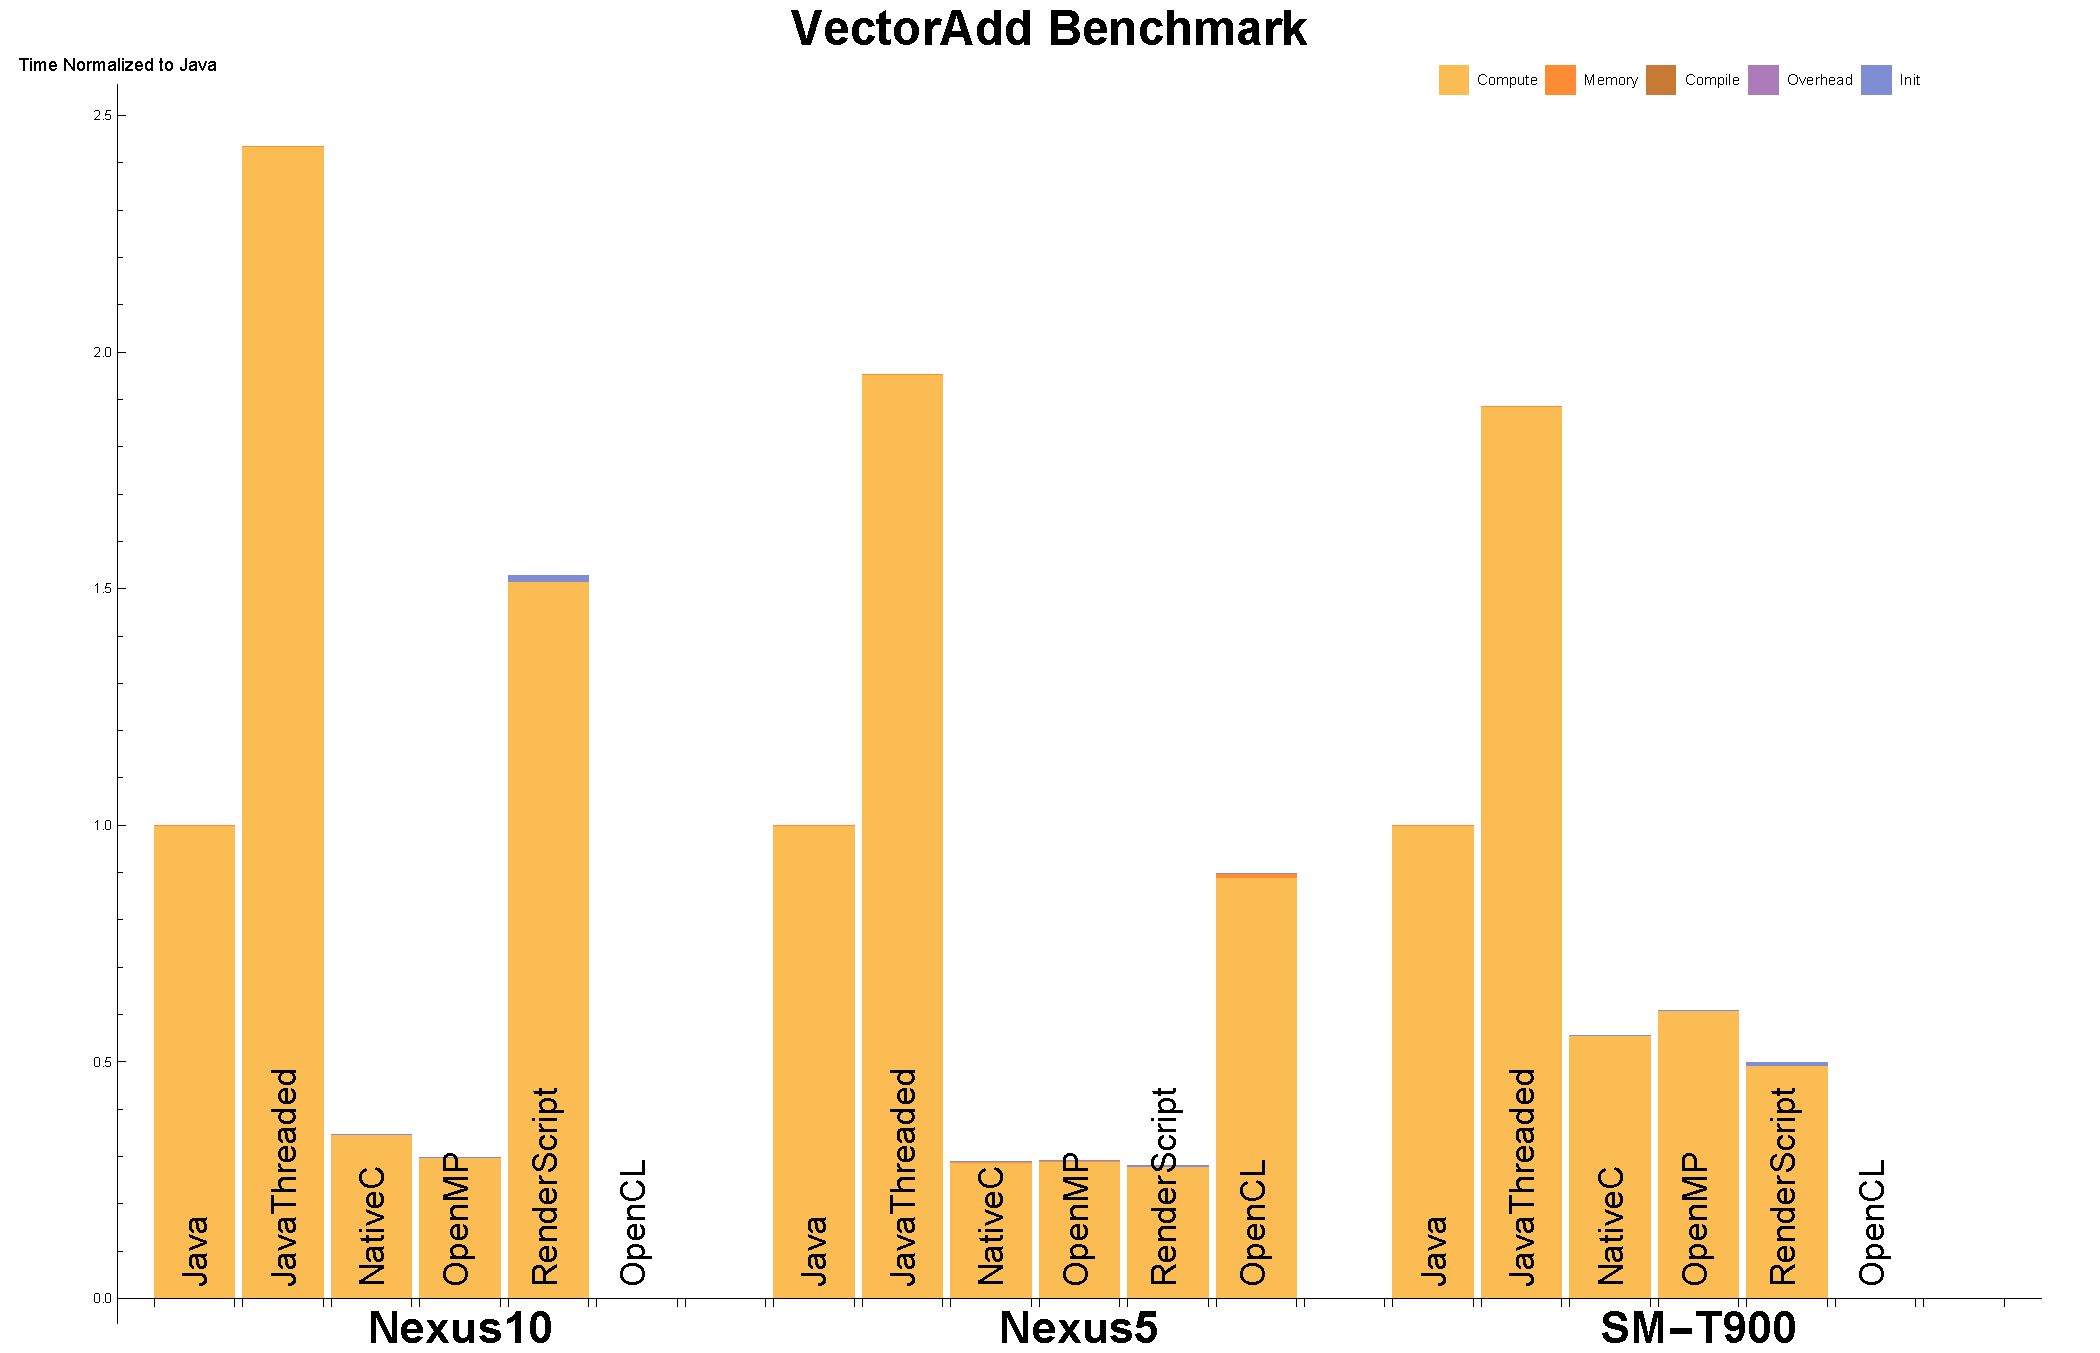
\includegraphics[width=0.9\textwidth]{data/VectorAdd_onecompute_time.pdf}
      \caption{VectorAdd}\label{fig:vectoradd}
  \end{subfigure}
  \begin{subfigure}[b]{0.5\textwidth}
      \centering
      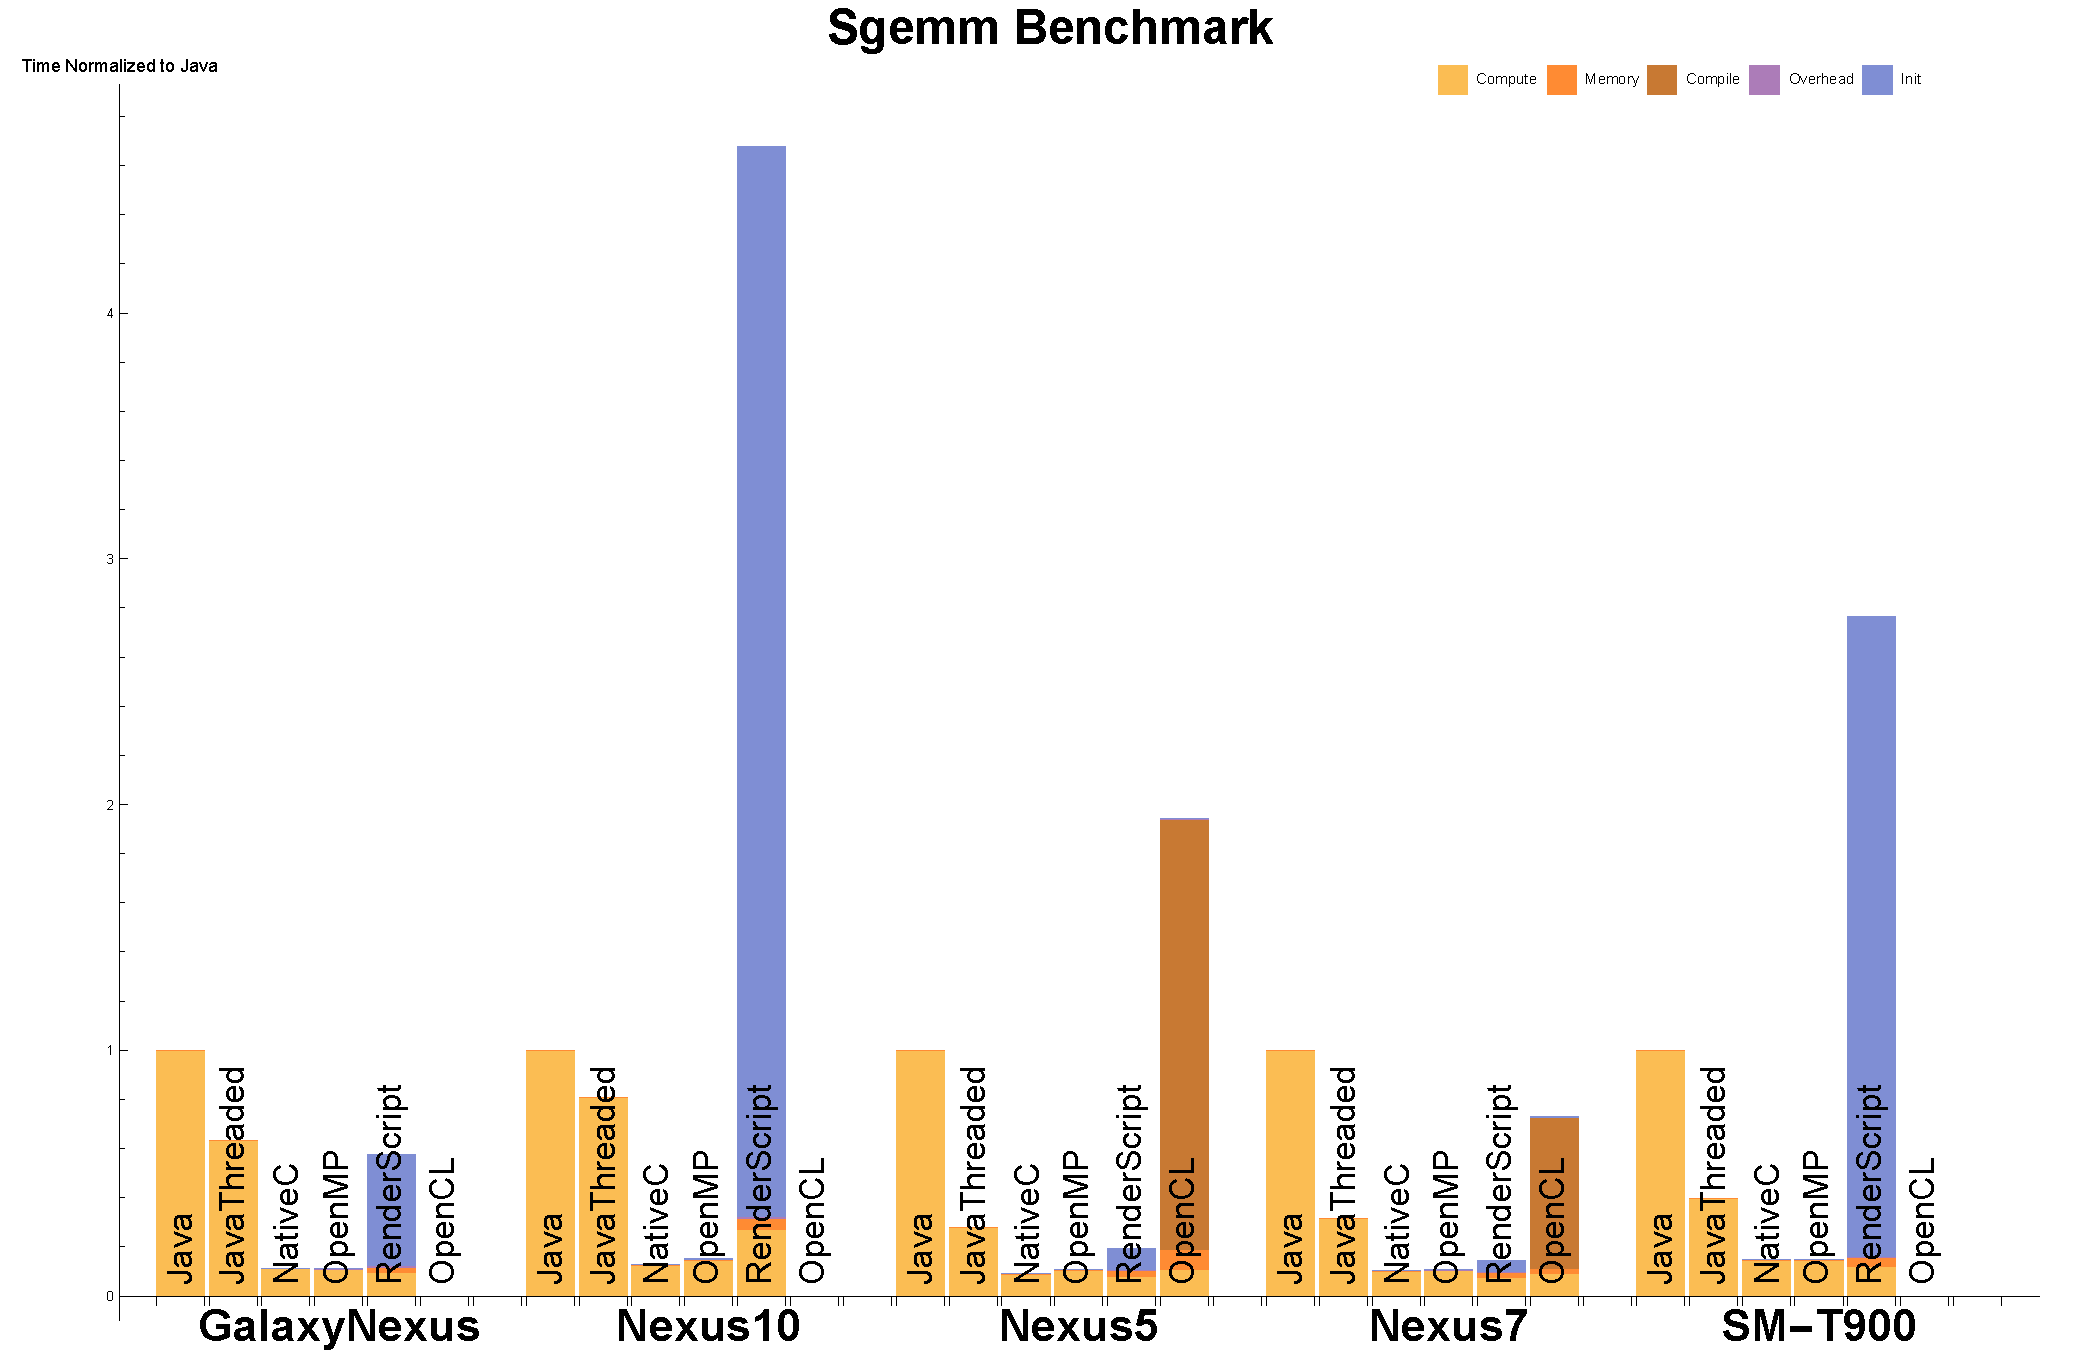
\includegraphics[width=0.9\textwidth]{data/Sgemm_onecompute_time.pdf}
      \caption{Sgemm}\label{fig:Sgemm}
  \end{subfigure}

  \begin{subfigure}[b]{0.5\textwidth}
      \centering
      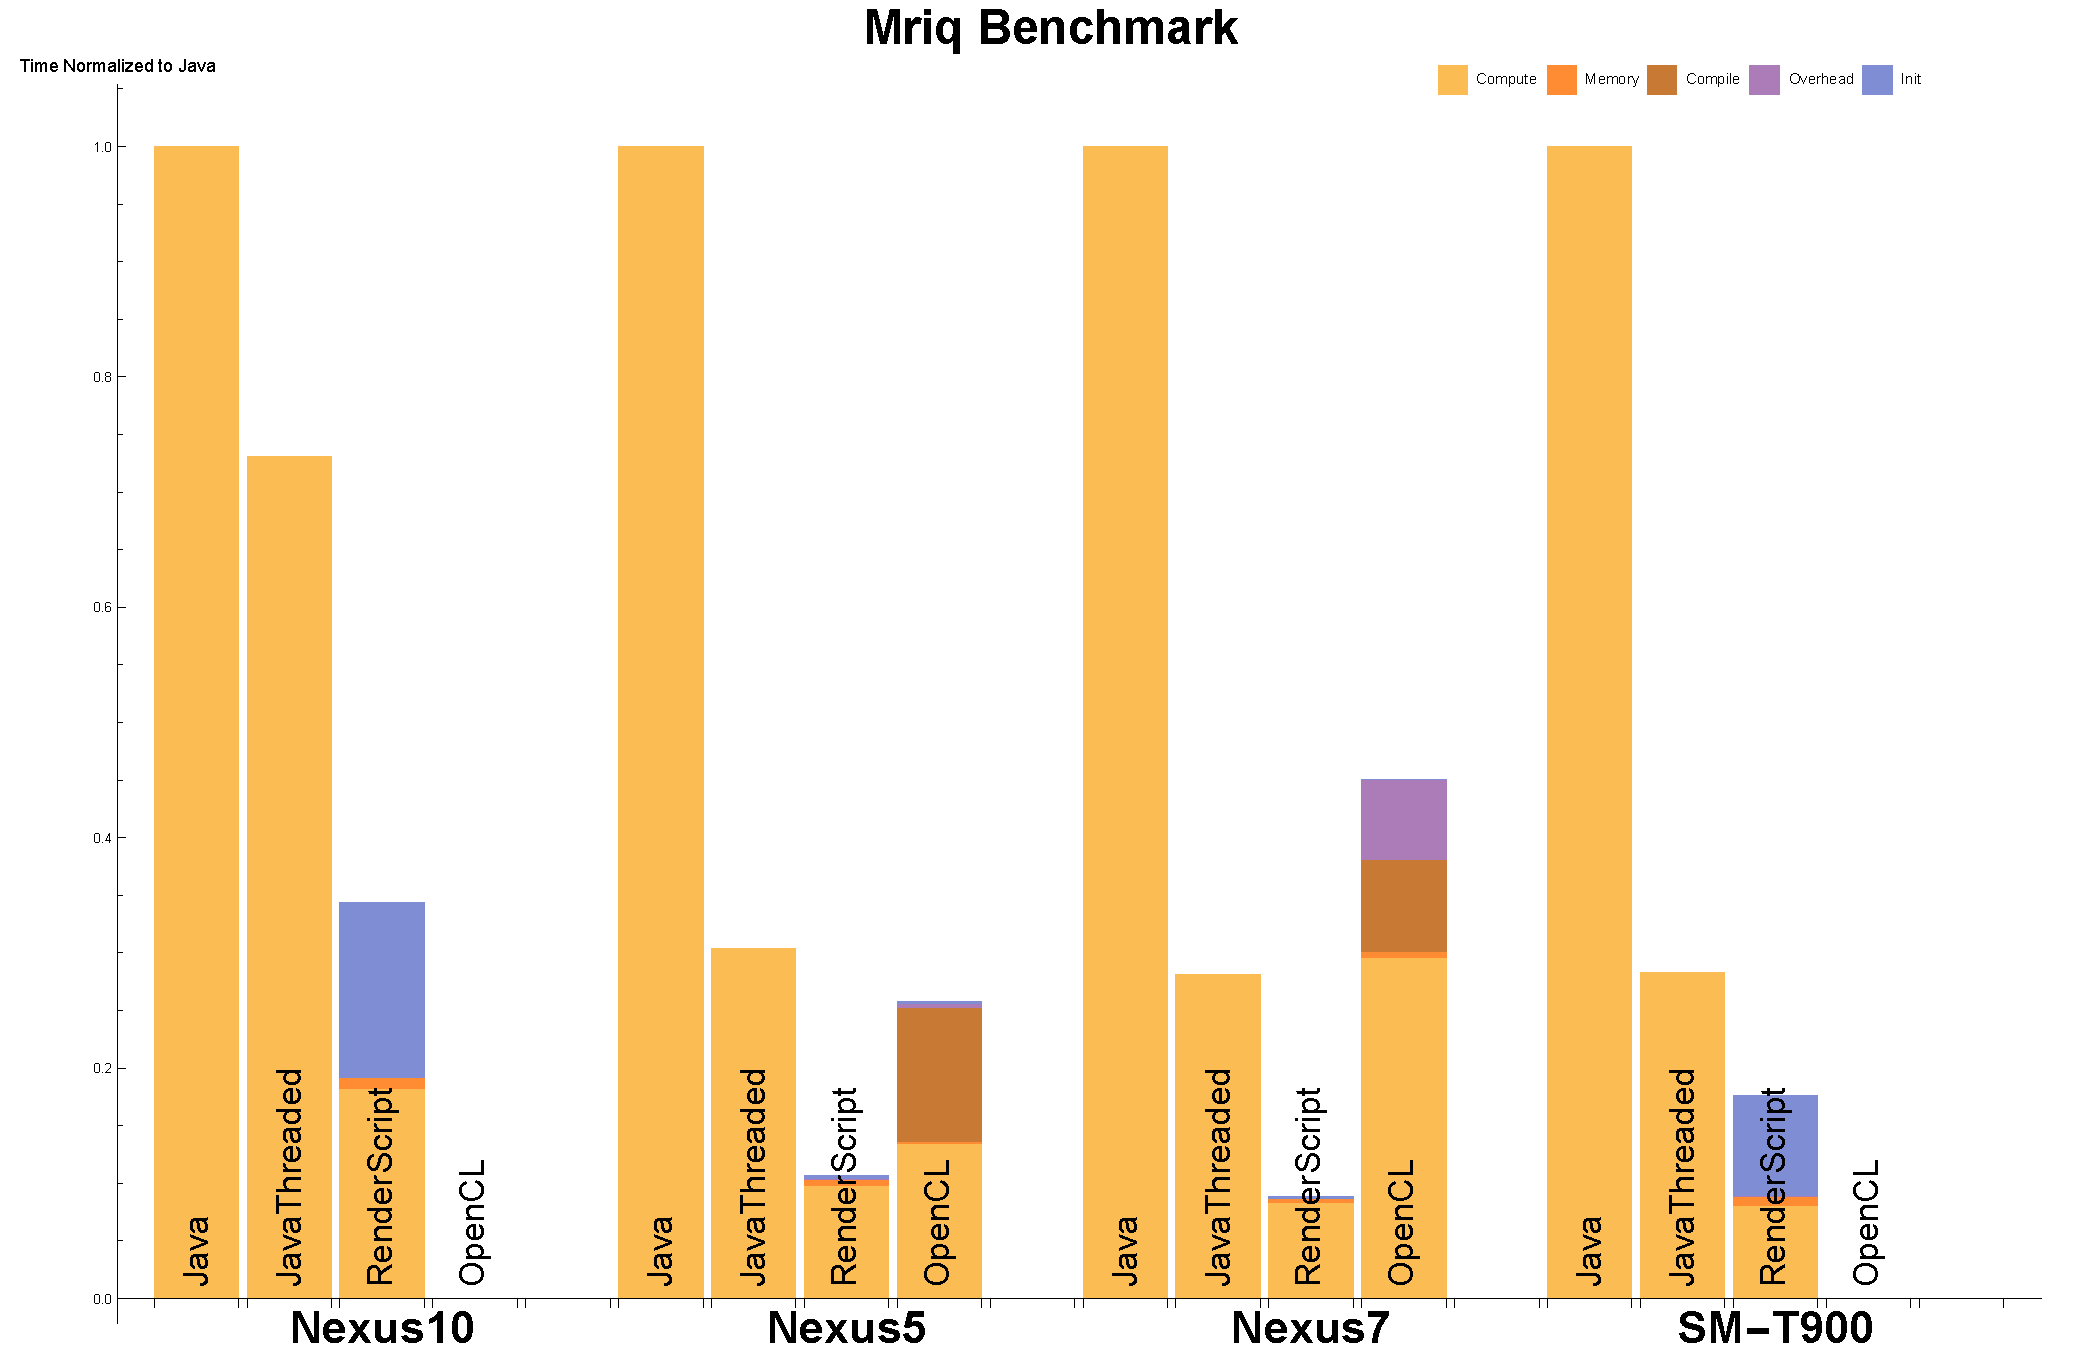
\includegraphics[width=0.9\textwidth]{data/Mriq_onecompute_time.pdf}
      \caption{MRIQ}
      \label{fig:MRIQ}
  \end{subfigure}
  \begin{subfigure}[b]{0.5\textwidth}
      \centering
      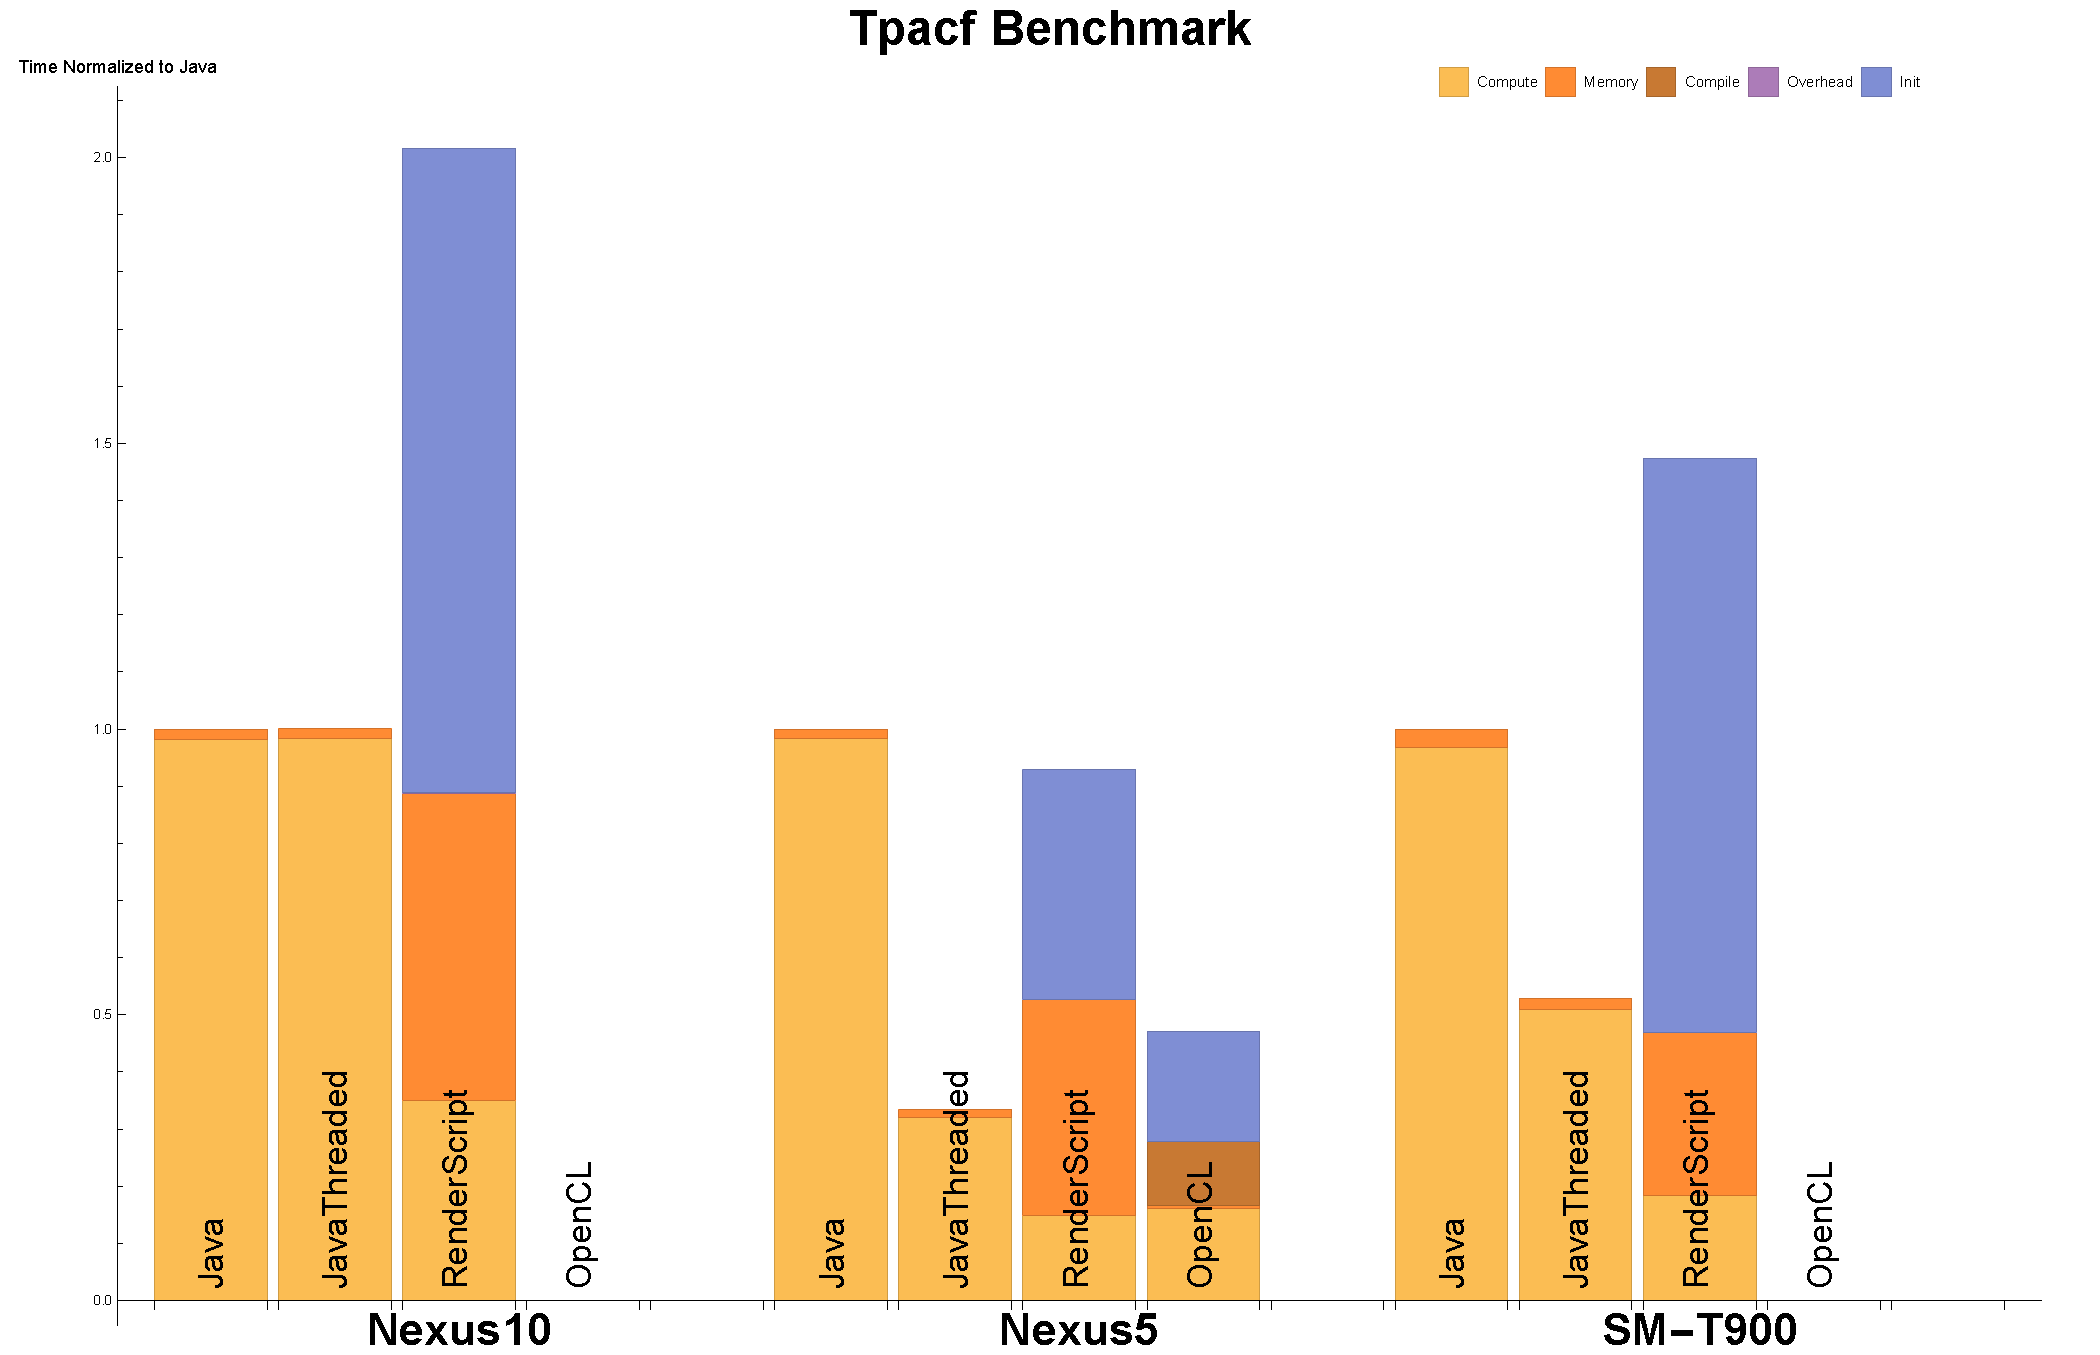
\includegraphics[width=0.9\textwidth]{data/Tpacf_onecompute_time.pdf}
      \caption{TPACF}
      \label{fig:TPACF}
  \end{subfigure}

  \begin{subfigure}[b]{0.5\textwidth}
      \centering
      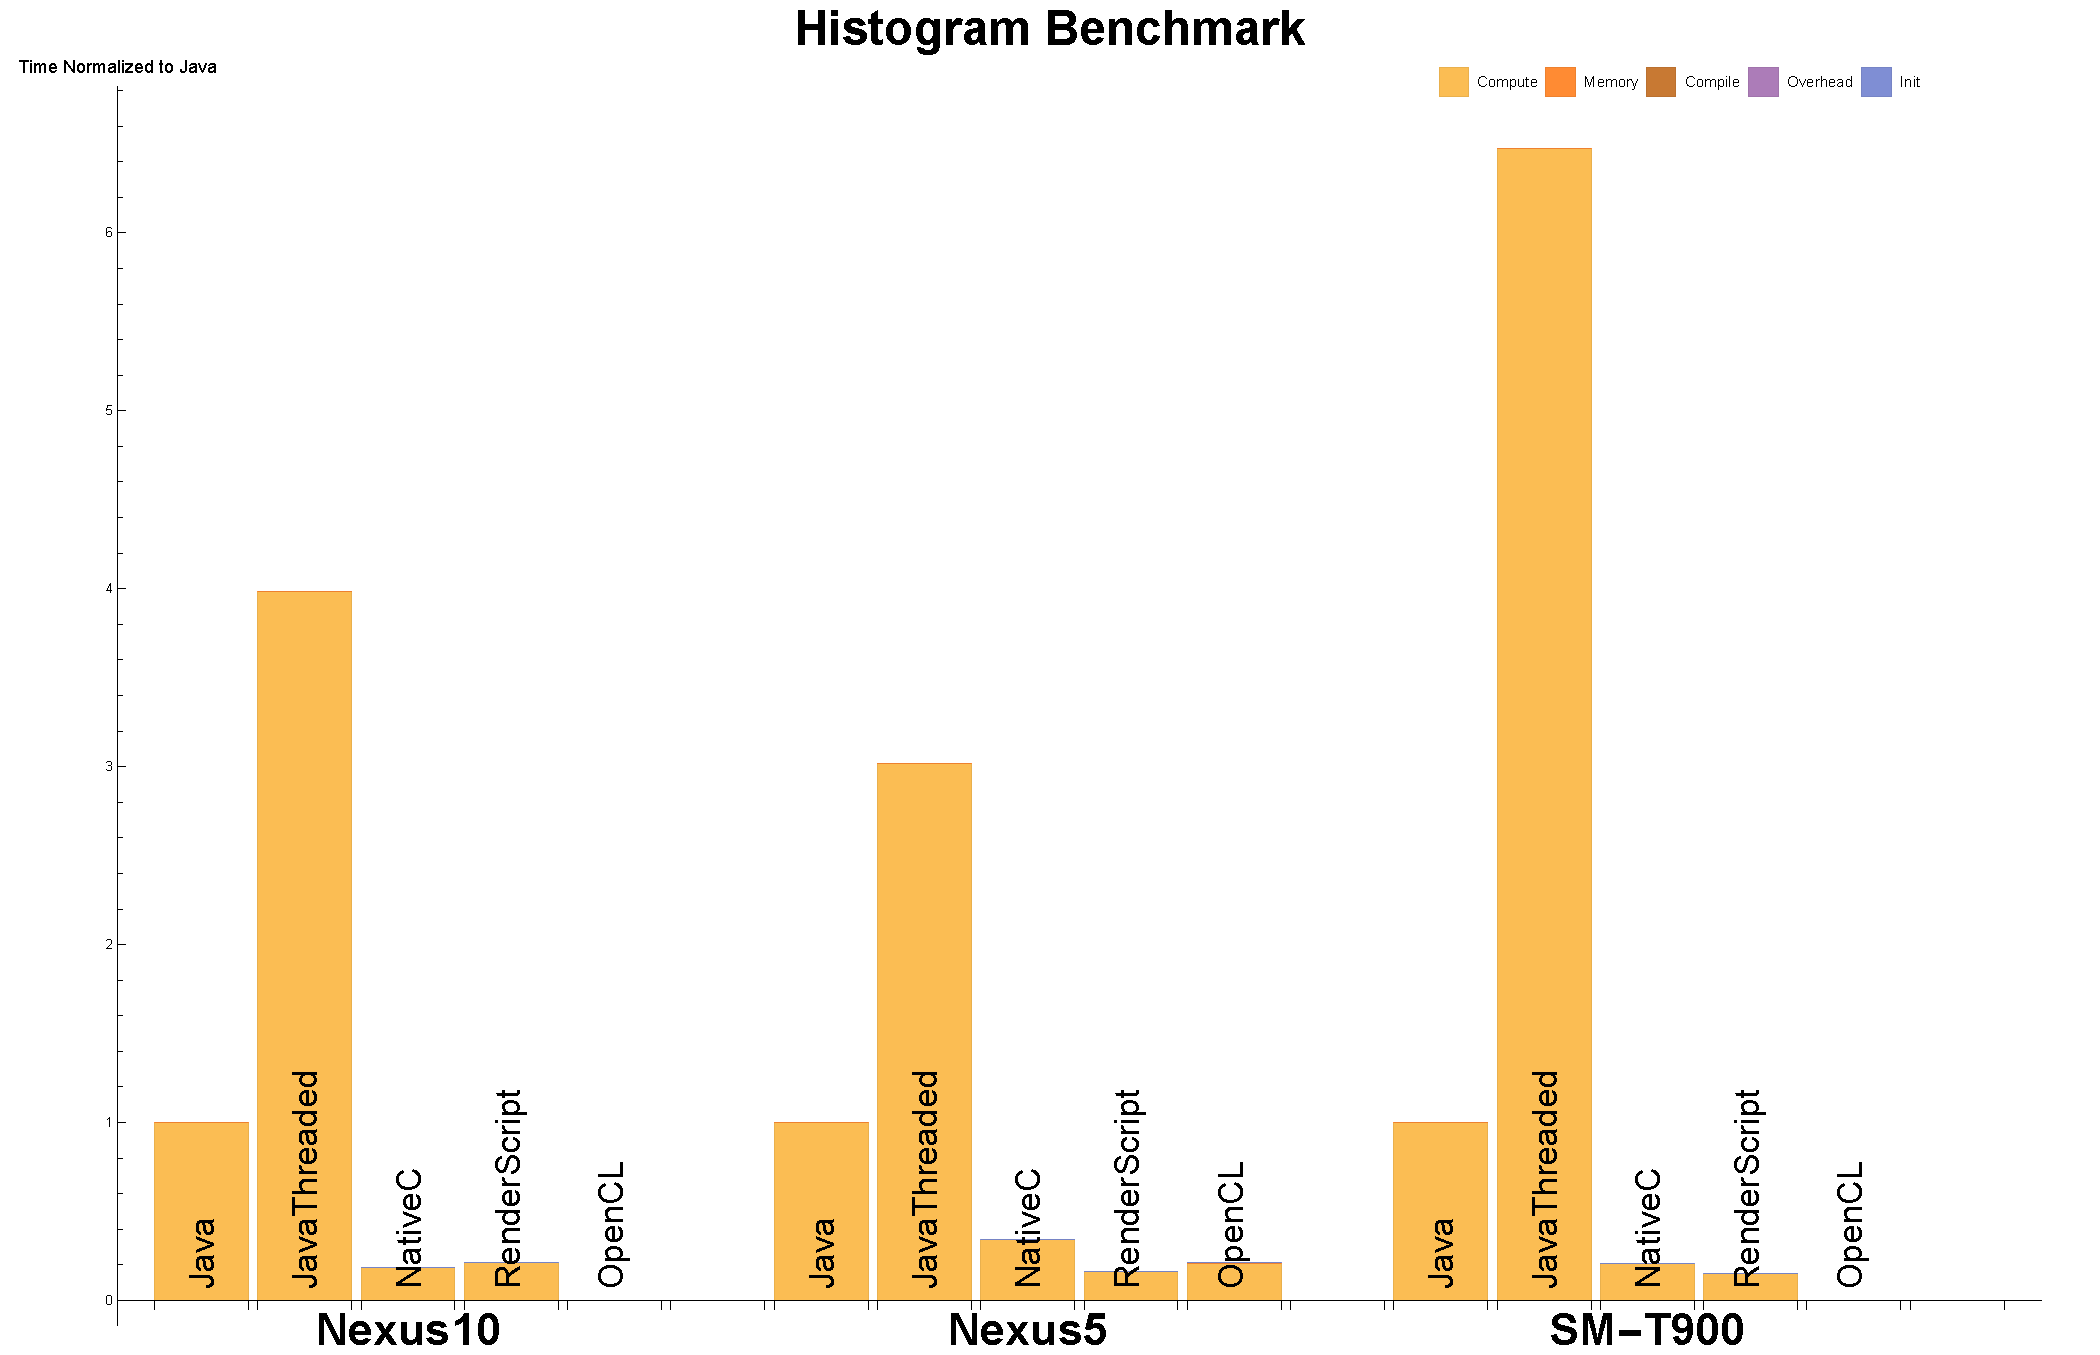
\includegraphics[width=0.9\textwidth]{data/Histogram_onecompute_time.pdf}
      \caption{Histogram}\label{fig:histo}
  \end{subfigure}
  \begin{subfigure}[b]{0.5\textwidth}
      \centering
      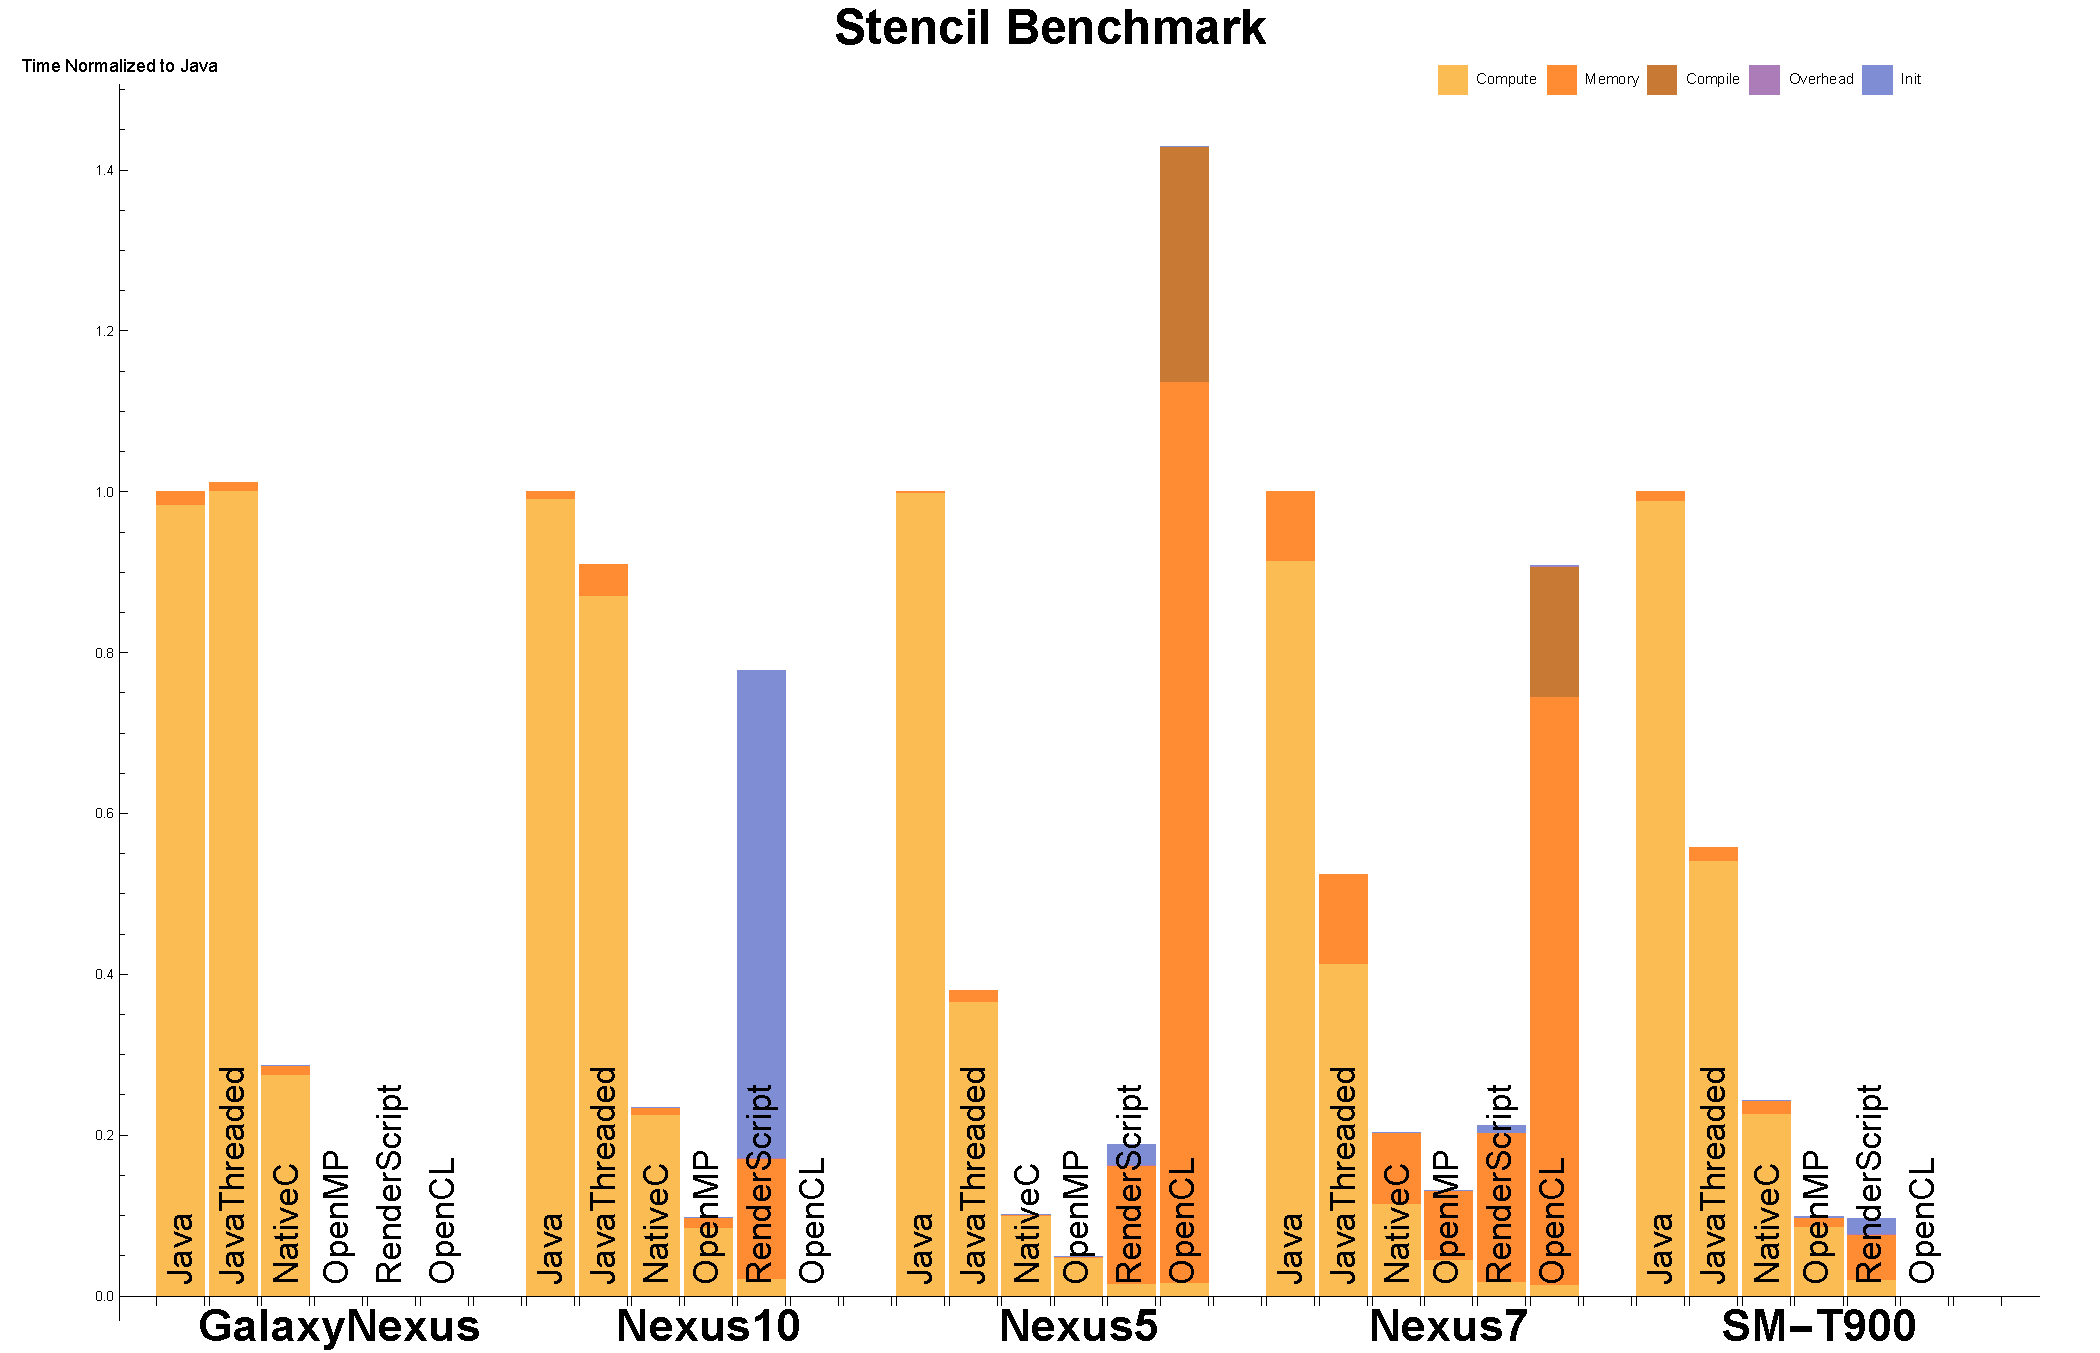
\includegraphics[width=0.9\textwidth]{data/Stencil_onecompute_time.pdf}
      \caption{Stencil}
      \label{fig:Stencil}
  \end{subfigure}

  \caption{Runtime across devices where kernel is exceuted once. J : Java, JT : JavaThreaded, C : C with JNI, OMP: OpenMP, OCL : OpenCL, and RS : Renderscript.}
\end{figure*}
\FloatBarrier

We evaluate each benchmark and its implementations on the devices listed
  in Table~\ref{table:hardware}.
The performance measurments are collected by measuring the time
  spent within each section of the code (as discussed in~\ref{design}).
The performance times are measured with the system connected to a
  power source, which avoids the device going to sleep (it does add the
  overhead of the device comunicating debug information with the development
  machine).

Each compute part of an implementation is run $5$ times with the minimum
  presented.
We consider two cases --- one where the kernel code is run once and therefore
  the overhead (memory, compilation, and initialization) have an impact,
  and one where the kernel is run $100$ times (or $5$ for both TPACF and MRIQ)
  and the overhead has little impact.

\todo[inline]{Discuss Performance.}


\subsubsection{Vector Add}

\subsubsection{SGEMM}

\subsubsection{TPACF}

\subsubsection{MRIQ}

\subsubsection{Stencil}

\subsubsection{Histogram}

\begin{figure*}[t]

  \begin{subfigure}[b]{\textwidth}
          \centering
          
\includegraphics[width=0.4\textwidth]{data/legend.pdf}
  \end{subfigure}

  \begin{subfigure}[b]{0.5\textwidth}
      \centering
      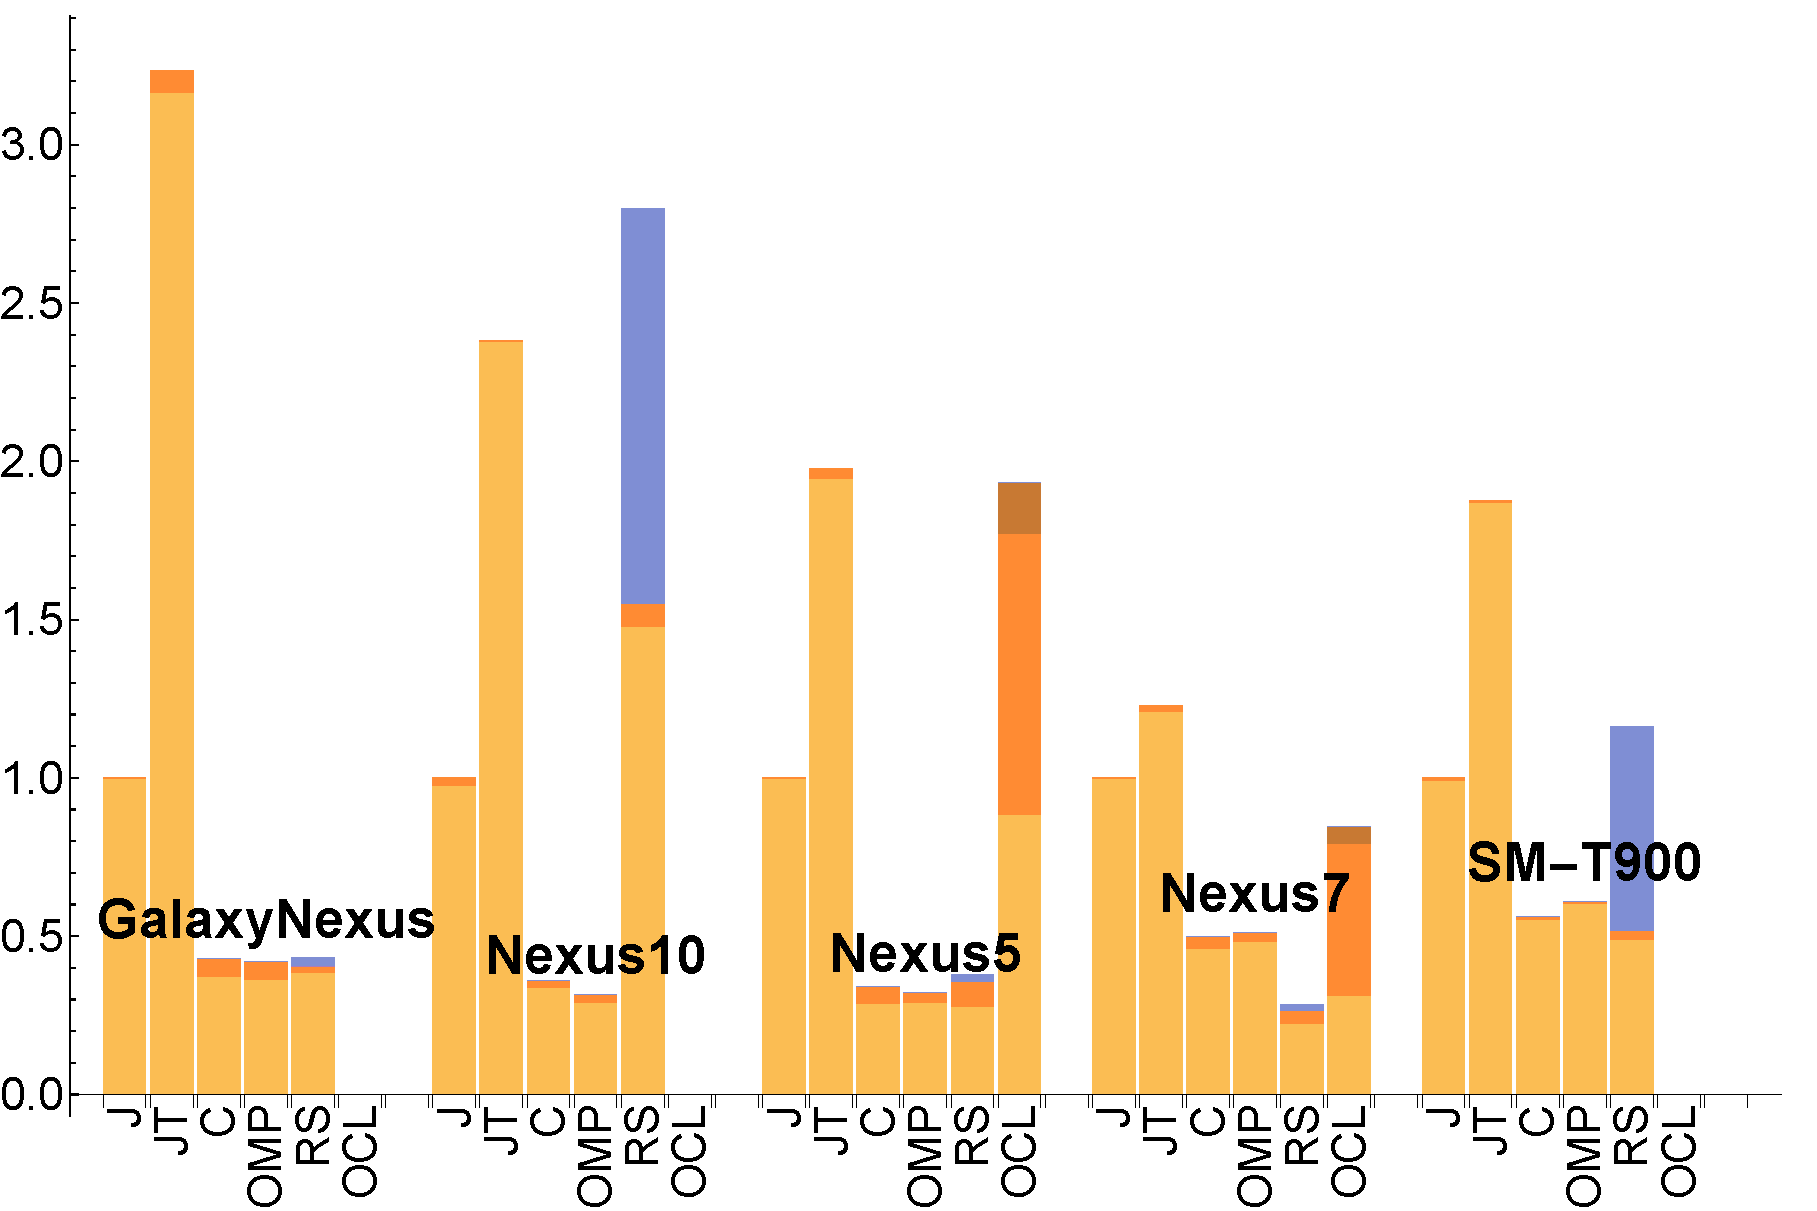
\includegraphics[width=0.9\textwidth]{data/VectorAdd_time.pdf}
      \caption{VectorAdd}\label{fig:vectoradd}
  \end{subfigure}
  \begin{subfigure}[b]{0.5\textwidth}
      \centering
      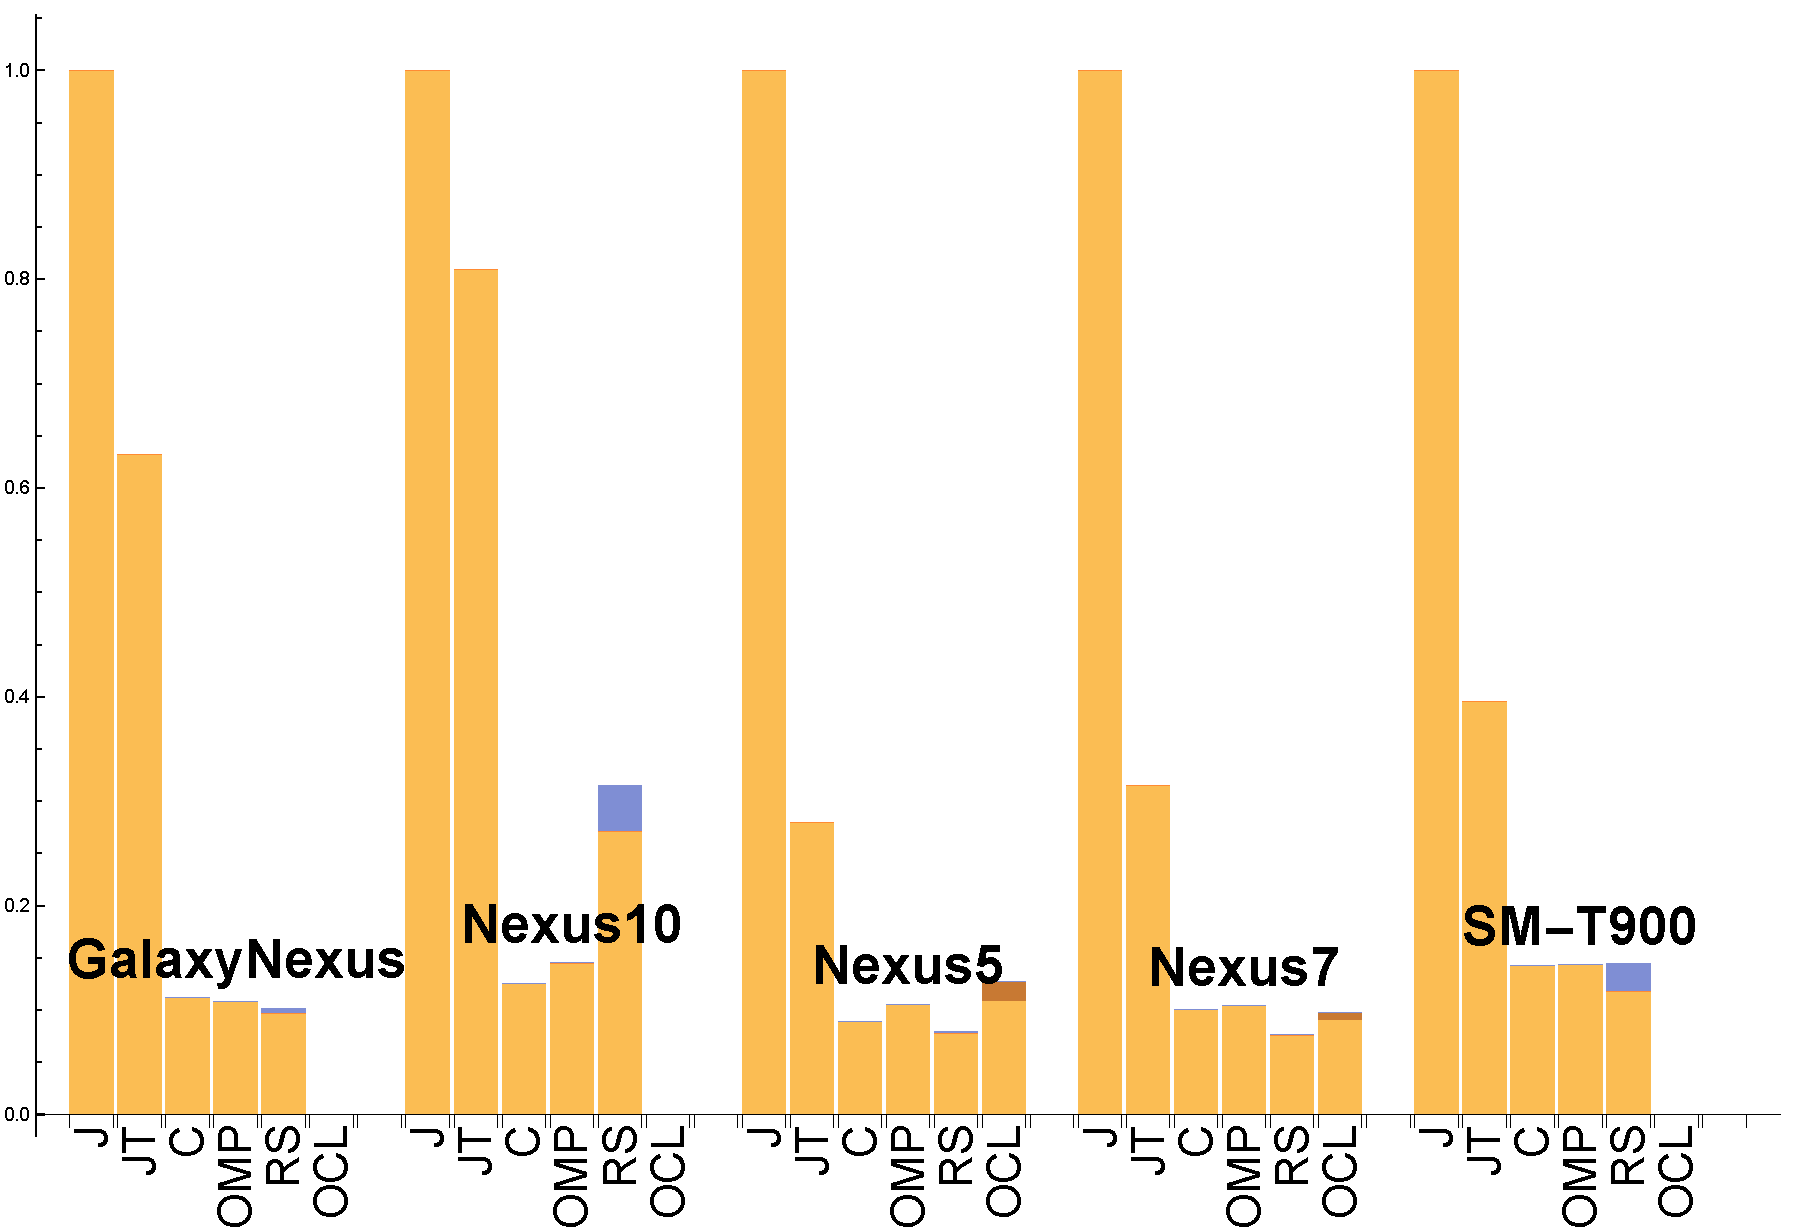
\includegraphics[width=0.9\textwidth]{data/Sgemm_time.pdf}
      \caption{Sgemm}\label{fig:Sgemm}
  \end{subfigure}

  \begin{subfigure}[b]{0.5\textwidth}
      \centering
      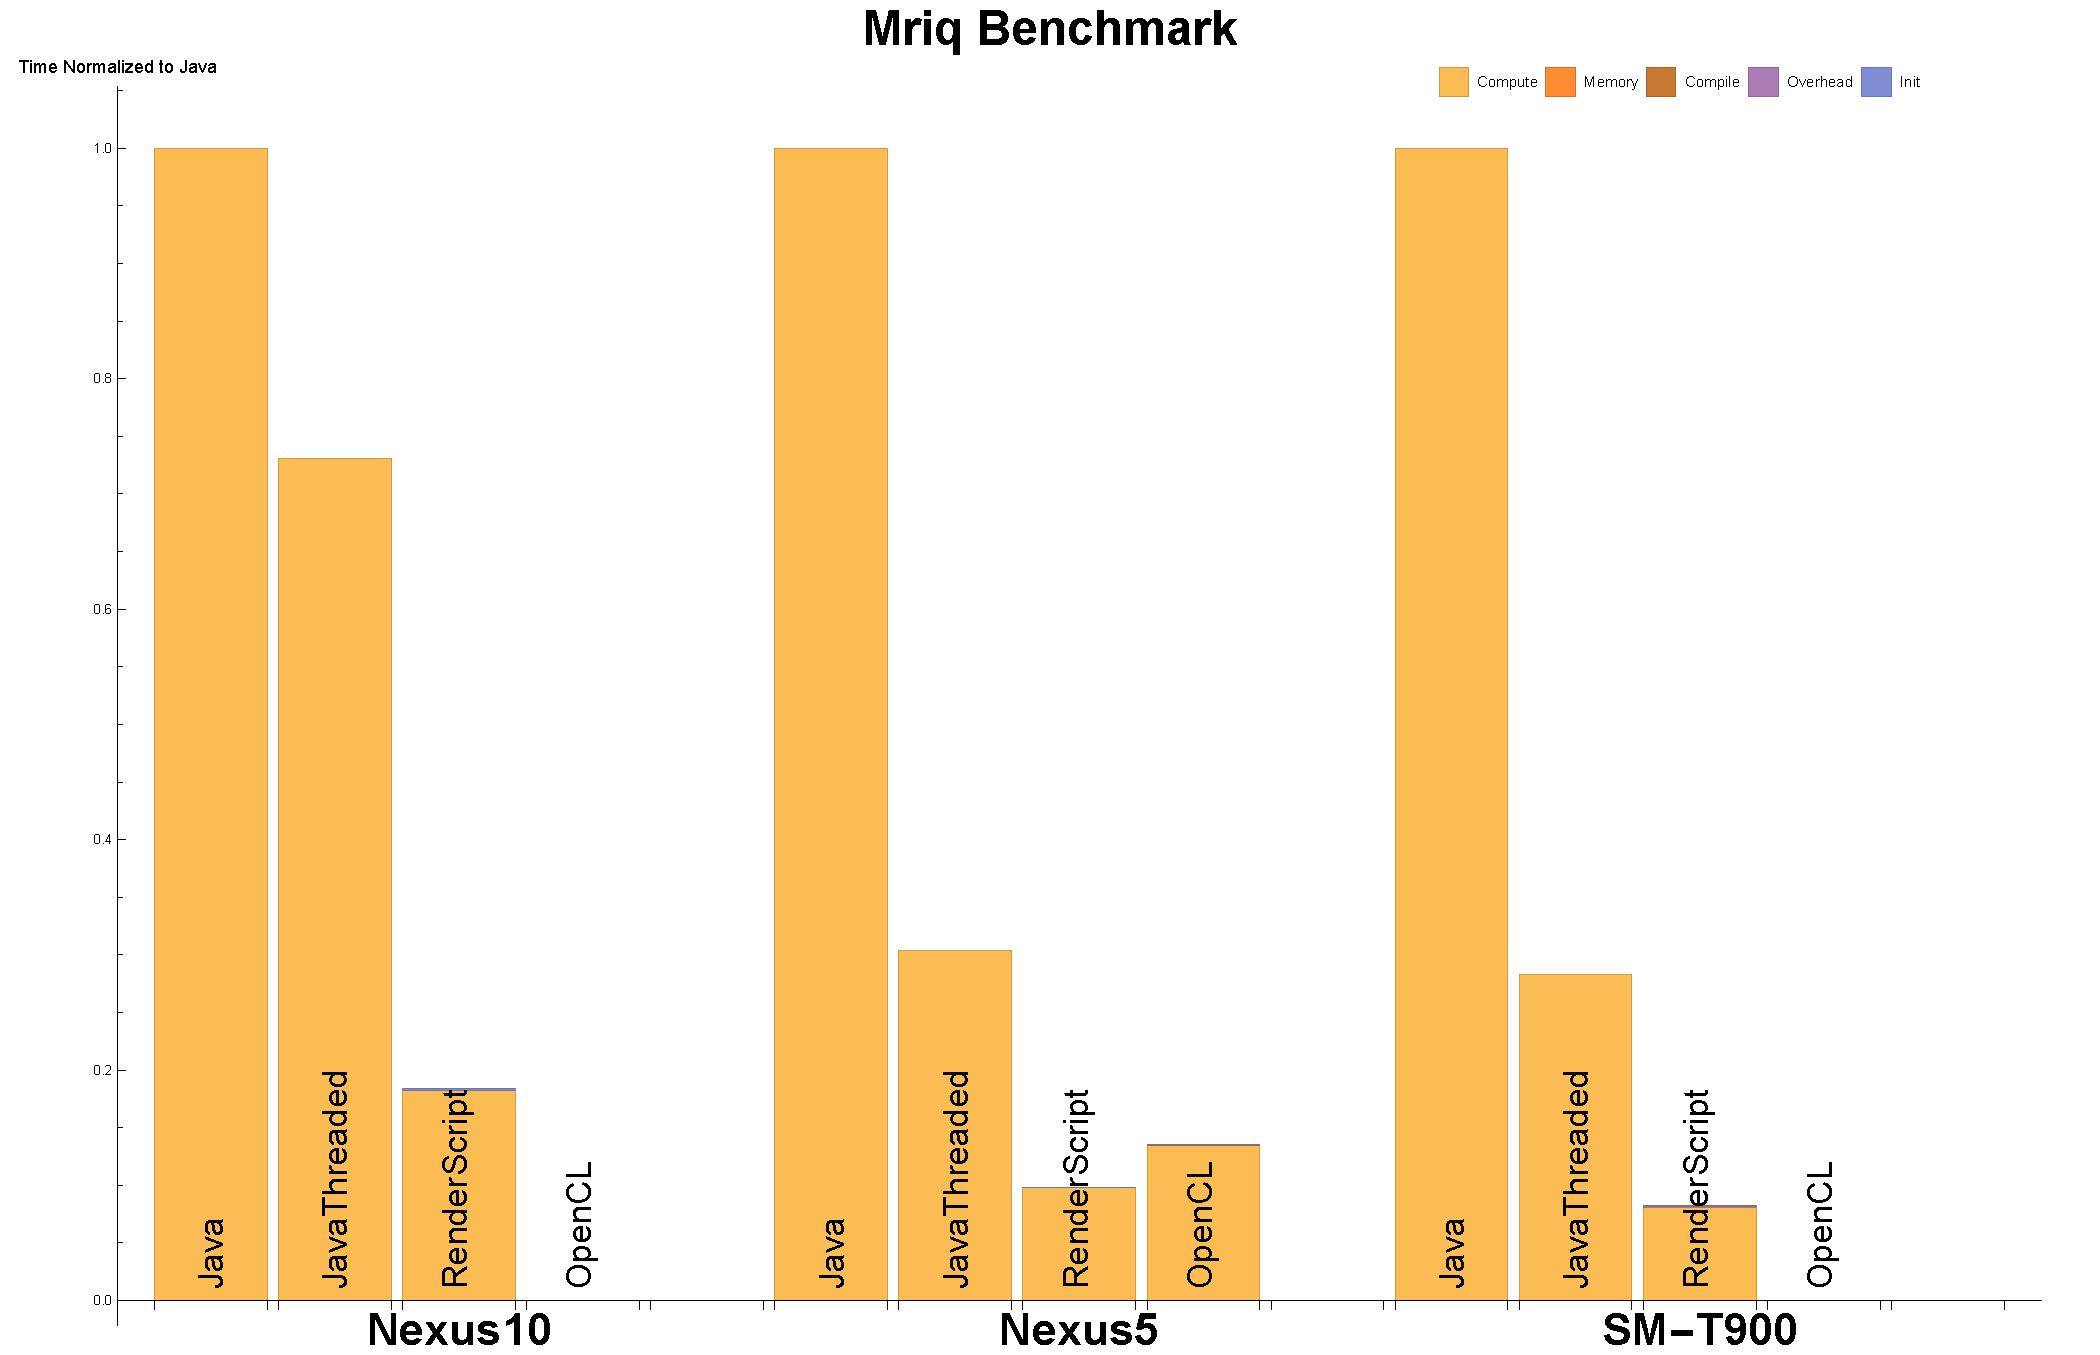
\includegraphics[width=0.9\textwidth]{data/Mriq_time.pdf}
      \caption{MRIQ}
      \label{fig:MRIQ}
  \end{subfigure}
  \begin{subfigure}[b]{0.5\textwidth}
      \centering
      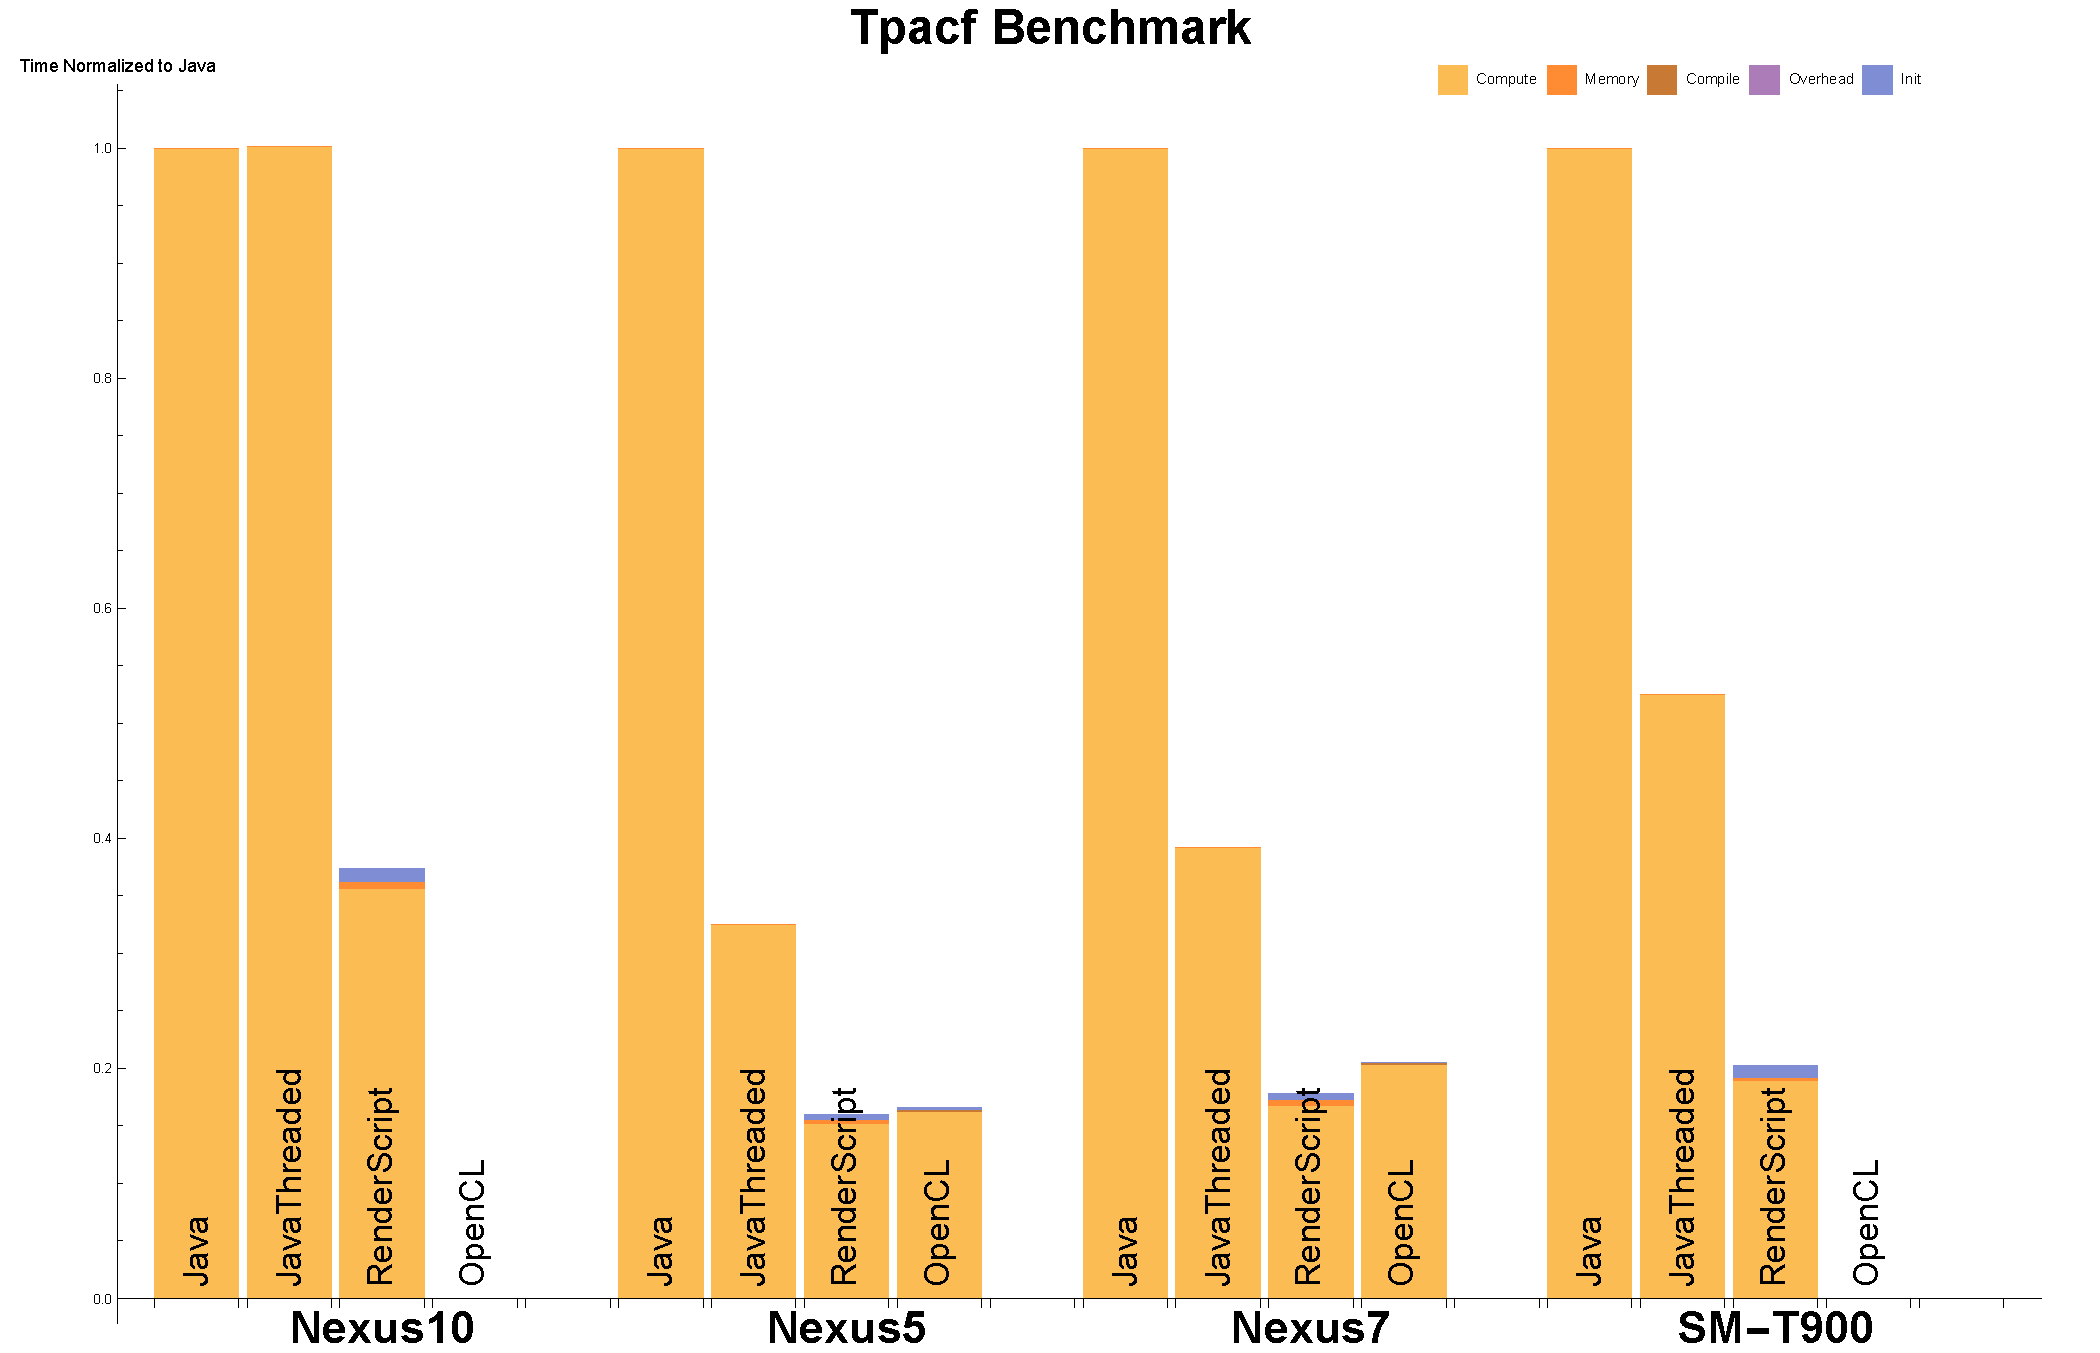
\includegraphics[width=0.9\textwidth]{data/Tpacf_time.pdf}
      \caption{TPACF}
      \label{fig:TPACF}
  \end{subfigure}

  \begin{subfigure}[b]{0.5\textwidth}
      \centering
      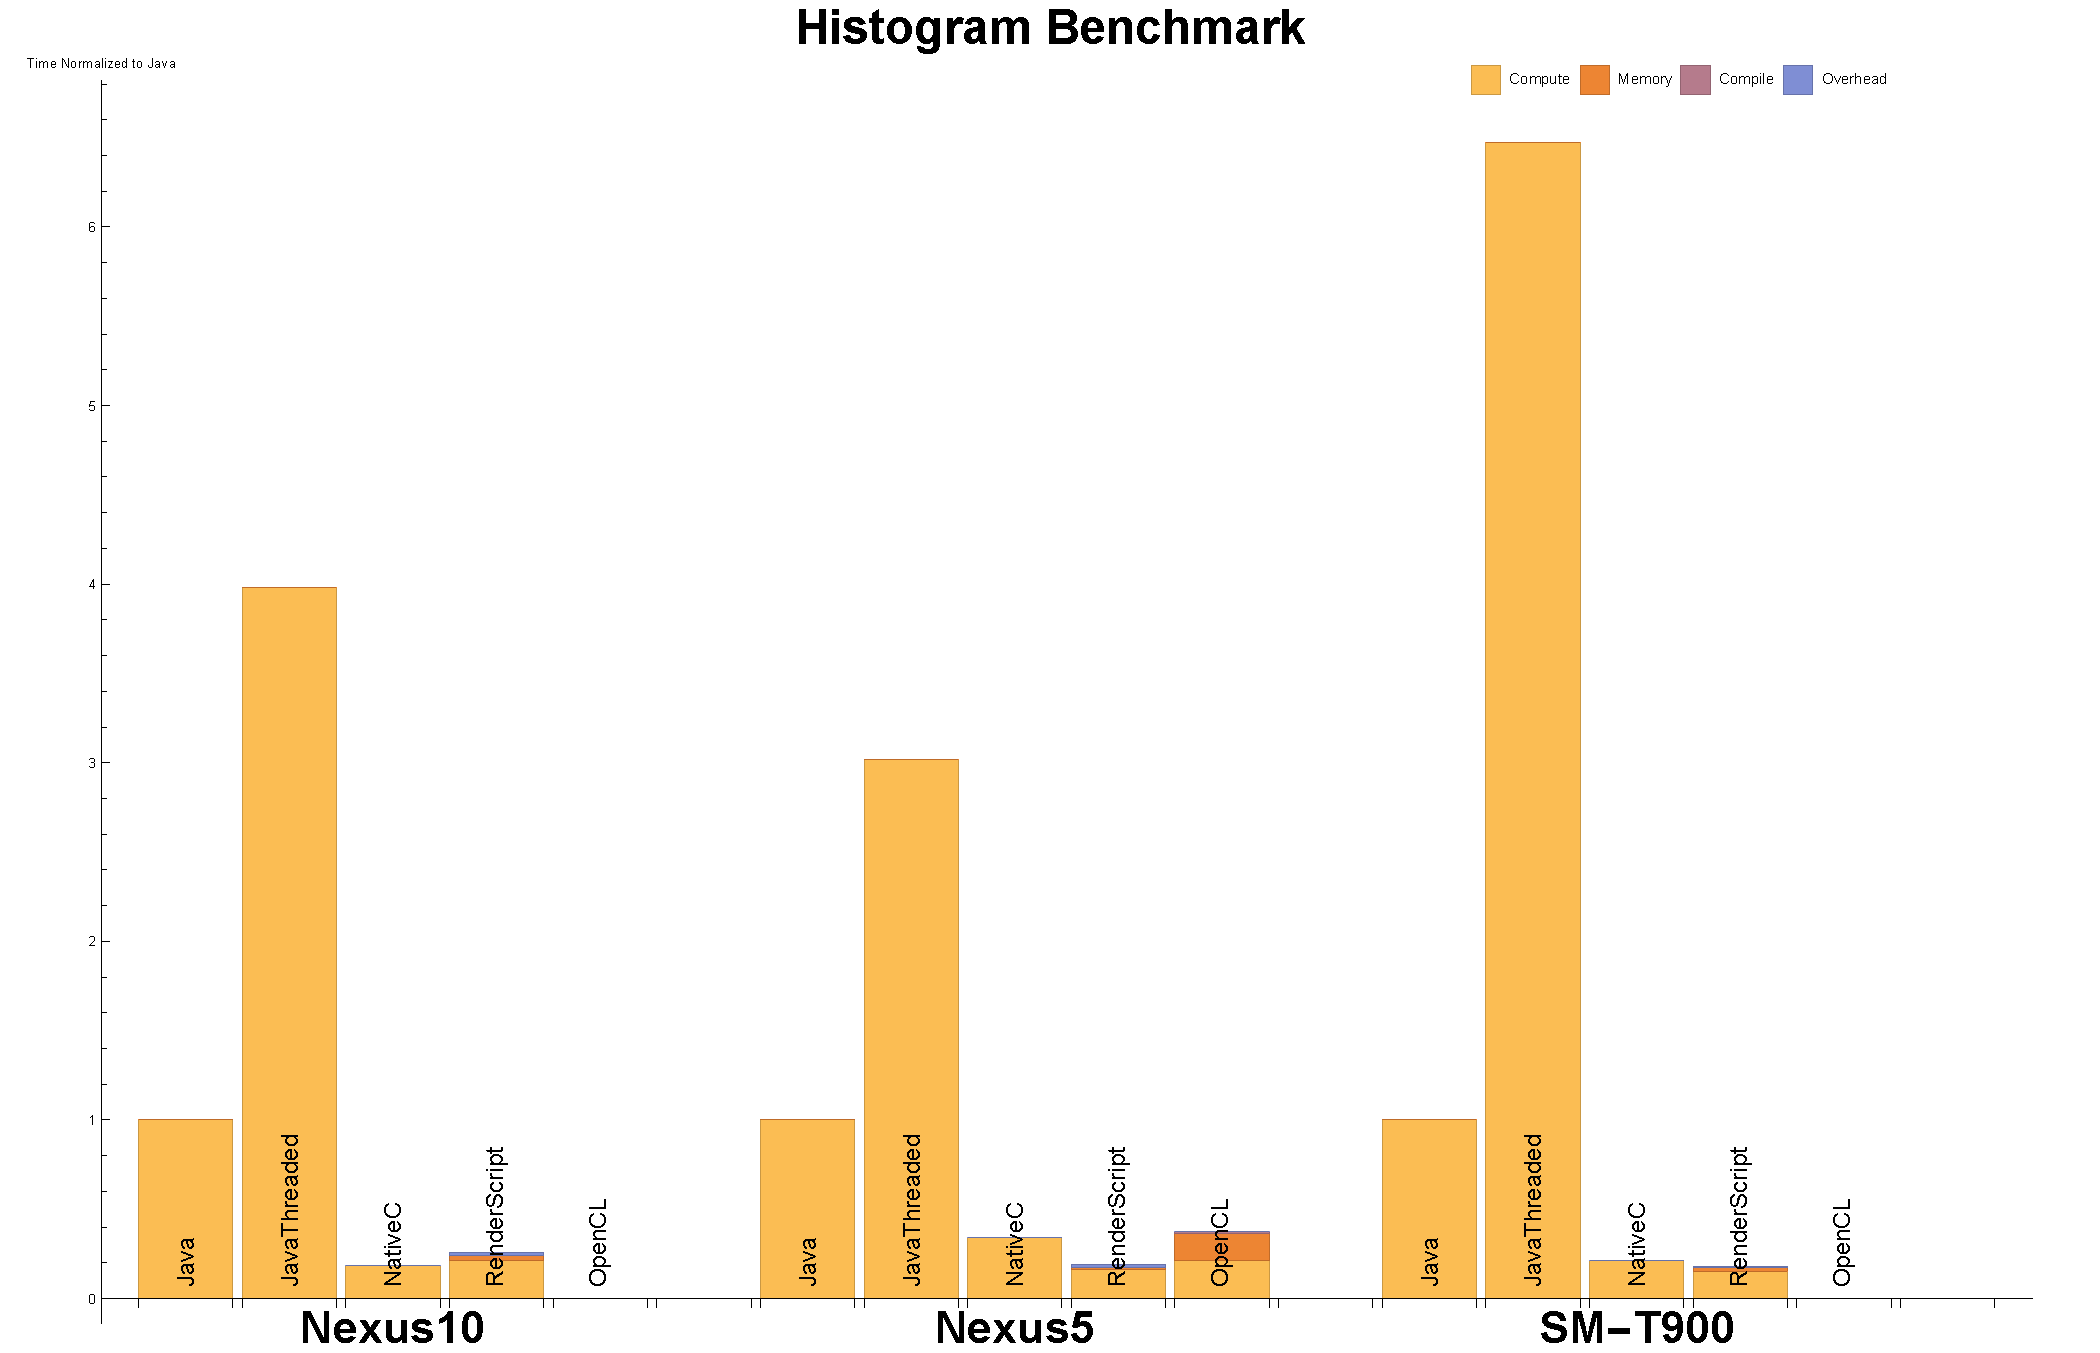
\includegraphics[width=0.9\textwidth]{data/Histogram_time.pdf}
      \caption{Histogram}\label{fig:histo}
  \end{subfigure}
  \begin{subfigure}[b]{0.5\textwidth}
      \centering
      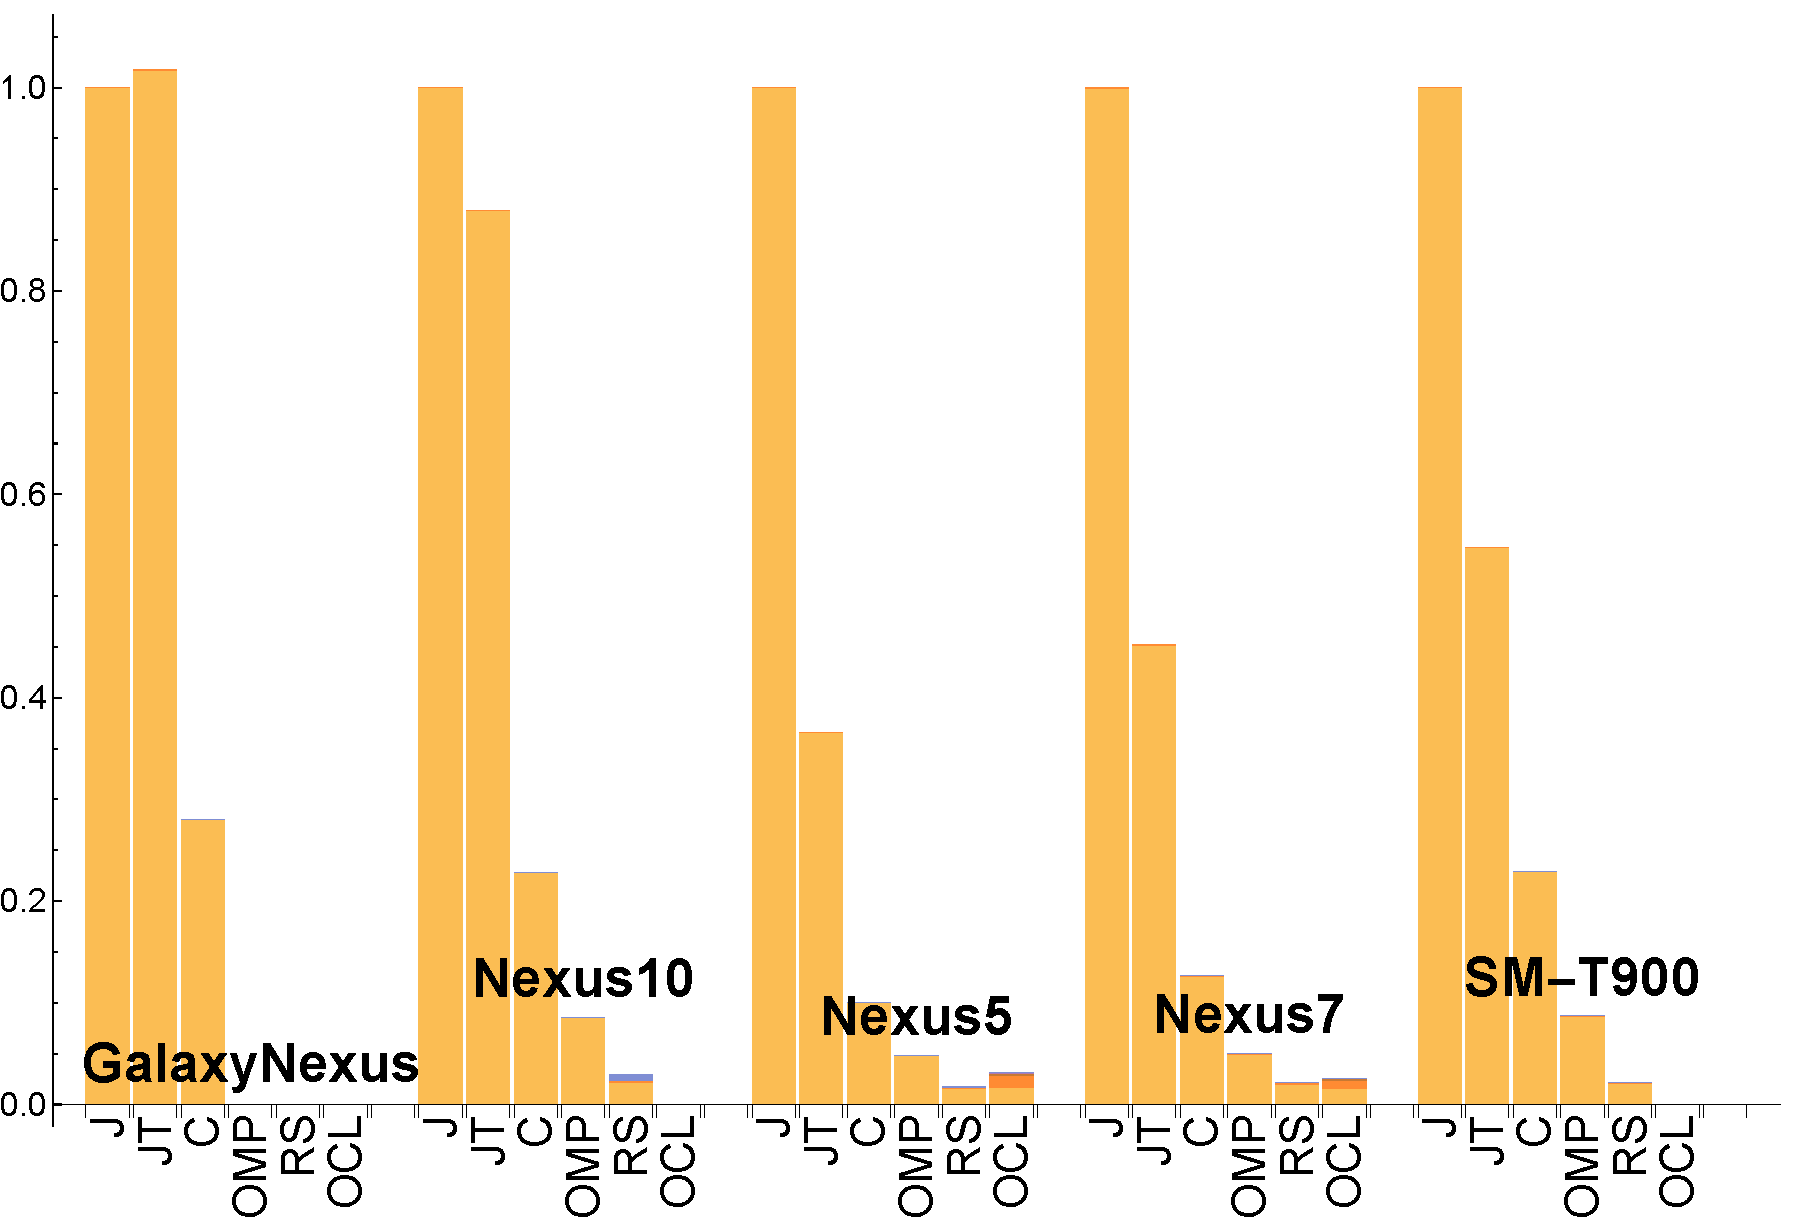
\includegraphics[width=0.9\textwidth]{data/Stencil_time.pdf}
      \caption{Stencil}
      \label{fig:Stencil}
  \end{subfigure}

  \caption{Runtime across devices where kernel is exceuted many times. J : Java, JT : JavaThreaded, C : C with JNI, OMP: OpenMP, OCL : OpenCL, and RS : Renderscript.}
\end{figure*}
\FloatBarrier